\documentclass{scrartcl}

%% support for CMYK color model. However, colors become bland when enabled
%\usepackage[natural]{xcolor}
%\usepackage[rgb]{pgf-cmykshadings}

%%
%% Libraries and packages used by the tikz files
%%

\usepackage{fdsymbol}

\usepackage{tikz}
\usepackage{ifthen}
\usepackage{circuitikz}

% listings package used for verbatim environments
\usepackage{listings}
\lstset{basicstyle=\ttfamily}

\usetikzlibrary{shapes,
                arrows,
                shadows.blur,
                fit,
                chains,
                fadings,
                patterns,
                decorations.pathmorphing,
                decorations.markings,
                shapes,
                scopes,
                backgrounds}

%%
%% TikZ fading definitions
%%

%%
% Fading used in timeline diagrams
%
\begin{tikzfadingfrompicture}[name=timeline fade right]
	\shade[left color=transparent!0,
	       right color=transparent!60] (0,0) rectangle (2,2);
\end{tikzfadingfrompicture}

%%
% Fading used in flow charts
%
\begin{tikzfadingfrompicture}[name=flow fade]
	\shade[left color=transparent!0,
	       right color=transparent!60] (0,0) rectangle (2,2);
\end{tikzfadingfrompicture}

\newcounter{decrhelper}


% A4: 21.0 × 29.7
\usepackage[paperwidth=21cm, paperheight=29.7cm]{geometry}

\begin{document}

../../img/tikz-common.tex

\begin{titlepage}
\thispagestyle{empty}

\begin{tikzpicture}[remember picture,overlay]

	\tikzstyle{section} = [minimum width=21cm, outer sep=0]
	\tikzstyle{user}    = [minimum width=5.25cm, minimum height=4cm, outer sep=0]

	\definecolor{techcolor}        {rgb}{0.6,0.7,0.9}
	\definecolor{sculptcolor}      {rgb}{0.4,0.3,0.4}
	\definecolor{innersculptcolor} {rgb}{0.5,0.4,0.5}
	\definecolor{ecosystemcolor}   {rgb}{0.7,0.9,0.6}
	\definecolor{usercolor}      {rgb}{0.8,0.45,0.52}
	\definecolor{innerusercolor} {rgb}{0.9,0.55,0.6}
	\definecolor{linkcolor}      {rgb}{0.0,0.1,0.6}

	%
	% Genode as technology
	%
	\path (current page.north)
		node[below=0cm, anchor=north, section, minimum height=6.5cm] (techoutline) {};

	\path (techoutline.west) -- coordinate[pos=0.5]  (mid)    (techoutline.east);
	\path (techoutline.west) -- coordinate[pos=0.4] (lefty)  (techoutline.east);
	\path (techoutline.west) -- coordinate[pos=0.6] (righty) (techoutline.east);

	\path (techoutline.south)+(0,5ex)  coordinate (southup);
	\path (techoutline.south)+(0,-0ex) coordinate (southdown);

	\tikzstyle{land} = [fill, inner color=white, path fading=flow fade, rounded corners=0]
	\path[land, opacity=0.4, outer color=techcolor]
		(techoutline.north west) --
		(techoutline.north east) --
		(techoutline.south east)
		.. controls +(-6ex,0ex) and +(6ex, 0ex) .. (righty |- southdown)
		.. controls +(-6ex,0ex) and +(6ex, 0ex) .. (mid    |- southup)
		.. controls +(-6ex,0ex) and +(6ex, 0ex) .. (lefty  |- southdown)
		.. controls +(-6ex,0ex) and +(6ex, 0ex) ..
		(techoutline.south west) --cycle;

	%
	% Sculpt OS as showcase
	%
	\path (techoutline.south)
		node[below=0cm, anchor=north, section, minimum height=13cm] (sculptoutline) {};

	\path (sculptoutline.north)+(0,5ex)  coordinate (northup);
	\path (sculptoutline.north)+(0,-0ex) coordinate (northdown);
	\path (sculptoutline.south)+(0,5ex)  coordinate (southup);
	\path (sculptoutline.south)+(0,-0ex) coordinate (southdown);

	\path[land, opacity=0.4, inner color=innersculptcolor, outer color=sculptcolor]
		(sculptoutline.north west)
		.. controls +(6ex,0ex) and +(-6ex, 0ex) .. (lefty  |- northdown)
		.. controls +(6ex,0ex) and +(-6ex, 0ex) .. (mid    |- northup)
		.. controls +(6ex,0ex) and +(-6ex, 0ex) .. (righty |- northdown)
		.. controls +(6ex,0ex) and +(-6ex, 0ex) ..
		(sculptoutline.north east) --
		(sculptoutline.south east)
		.. controls +(-6ex,0ex) and +(6ex, 0ex) .. (righty |- southdown)
		.. controls +(-6ex,0ex) and +(6ex, 0ex) .. (mid    |- southup)
		.. controls +(-6ex,0ex) and +(6ex, 0ex) .. (lefty  |- southdown)
		.. controls +(-6ex,0ex) and +(6ex, 0ex) ..
		(sculptoutline.south west) --cycle;

	%
	% Ecosystem
	%
	\path (sculptoutline.south)
		node[below=0cm, anchor=north, section, minimum height=6.5cm] (ecooutline) {};

	\path (ecooutline.north)+(0,5ex)  coordinate (northup);
	\path (ecooutline.north)+(0,-0ex) coordinate (northdown);
	\path (ecooutline.south)+(0,5ex)  coordinate (southup);
	\path (ecooutline.south)+(0,-0ex) coordinate (southdown);

	\path (techoutline.west) --
		coordinate[pos=0]    (p1west) coordinate[pos=0.25] (p1east)
		coordinate[pos=0.25] (p2west) coordinate[pos=0.5]  (p2east)
		coordinate[pos=0.5]  (p3west) coordinate[pos=0.75] (p3east)
		coordinate[pos=0.75] (p4west) coordinate[pos=1]    (p4east)
		(techoutline.east);

	\path (p1west) -- coordinate[pos=0.5]  (p1mid)    (p1east);
	\path (p1west) -- coordinate[pos=0.25] (p1lefty)  (p1east);
	\path (p1west) -- coordinate[pos=0.75] (p1righty) (p1east);

	\path (p2west) -- coordinate[pos=0.5]  (p2mid)    (p2east);
	\path (p2west) -- coordinate[pos=0.25] (p2lefty)  (p2east);
	\path (p2west) -- coordinate[pos=0.75] (p2righty) (p2east);

	\path (p3west) -- coordinate[pos=0.5]  (p3mid)    (p3east);
	\path (p3west) -- coordinate[pos=0.25] (p3lefty)  (p3east);
	\path (p3west) -- coordinate[pos=0.75] (p3righty) (p3east);

	\path (p4west) -- coordinate[pos=0.5]  (p4mid)    (p4east);
	\path (p4west) -- coordinate[pos=0.25] (p4lefty)  (p4east);
	\path (p4west) -- coordinate[pos=0.75] (p4righty) (p4east);

	\path[land, opacity=0.4, outer color=ecosystemcolor]
		(ecooutline.north west)
		.. controls +(6ex,0ex) and +(-6ex, 0ex) .. (lefty  |- northdown)
		.. controls +(6ex,0ex) and +(-6ex, 0ex) .. (mid    |- northup)
		.. controls +(6ex,0ex) and +(-6ex, 0ex) .. (righty |- northdown)
		.. controls +(6ex,0ex) and +(-6ex, 0ex) ..
		(ecooutline.north east) --
		(ecooutline.south east)
		.. controls +(-4ex,0ex) and +(4ex, 0ex) .. (p4righty |- southdown)
		.. controls +(-4ex,0ex) and +(4ex, 0ex) .. (p4mid    |- southup)
		.. controls +(-4ex,0ex) and +(4ex, 0ex) .. (p4lefty  |- southdown)
		.. controls +(-4ex,0ex) and +(4ex, 0ex) .. (p4west |- ecooutline.south)

		.. controls +(-4ex,0ex) and +(4ex, 0ex) .. (p3righty |- southdown)
		.. controls +(-4ex,0ex) and +(4ex, 0ex) .. (p3mid    |- southup)
		.. controls +(-4ex,0ex) and +(4ex, 0ex) .. (p3lefty  |- southdown)
		.. controls +(-4ex,0ex) and +(4ex, 0ex) .. (p3west |- ecooutline.south)

		.. controls +(-4ex,0ex) and +(4ex, 0ex) .. (p2righty |- southdown)
		.. controls +(-4ex,0ex) and +(4ex, 0ex) .. (p2mid    |- southup)
		.. controls +(-4ex,0ex) and +(4ex, 0ex) .. (p2lefty  |- southdown)
		.. controls +(-4ex,0ex) and +(4ex, 0ex) .. (p2west |- ecooutline.south)

		.. controls +(-4ex,0ex) and +(4ex, 0ex) .. (p1righty |- southdown)
		.. controls +(-4ex,0ex) and +(4ex, 0ex) .. (p1mid    |- southup)
		.. controls +(-4ex,0ex) and +(4ex, 0ex) .. (p1lefty  |- southdown)
		.. controls +(-4ex,0ex) and +(4ex, 0ex) .. (p1west |- ecooutline.south)
		--
		(ecooutline.south west) --cycle;


	\path (p1mid |- ecooutline.south) node[below=0cm, anchor=north, user] (vendoroutline) { };
	\path (p2mid |- ecooutline.south) node[below=0cm, anchor=north, user] (oemoutline) { };
	\path (p3mid |- ecooutline.south) node[below=0cm, anchor=north, user] (productoutline) { };
	\path (p4mid |- ecooutline.south) node[below=0cm, anchor=north, user] (researchoutline) { };

	\path (vendoroutline.north)+(0,5ex)  coordinate (northup);
	\path (vendoroutline.north)+(0,-0ex) coordinate (northdown);

	\path[land, opacity=0.5, inner color=innerusercolor, outer color=usercolor]
		(vendoroutline.north west)
		.. controls +(4ex,0ex) and +(-4ex, 0ex) .. (p1lefty  |- northdown)
		.. controls +(4ex,0ex) and +(-4ex, 0ex) .. (p1mid    |- northup)
		.. controls +(4ex,0ex) and +(-4ex, 0ex) .. (p1righty |- northdown)
		.. controls +(4ex,0ex) and +(-4ex, 0ex) ..
		(vendoroutline.north east) -- (vendoroutline.south east) --
		(vendoroutline.south west) --cycle;

	\path[land, opacity=0.48, inner color=innerusercolor, outer color=usercolor]
		(oemoutline.north west)
		.. controls +(4ex,0ex) and +(-4ex, 0ex) .. (p2lefty  |- northdown)
		.. controls +(4ex,0ex) and +(-4ex, 0ex) .. (p2mid    |- northup)
		.. controls +(4ex,0ex) and +(-4ex, 0ex) .. (p2righty |- northdown)
		.. controls +(4ex,0ex) and +(-4ex, 0ex) ..
		(oemoutline.north east) -- (oemoutline.south east) --
		(oemoutline.south west) --cycle;

	\path[land, opacity=0.45, inner color=innerusercolor, outer color=usercolor]
		(productoutline.north west)
		.. controls +(4ex,0ex) and +(-4ex, 0ex) .. (p3lefty  |- northdown)
		.. controls +(4ex,0ex) and +(-4ex, 0ex) .. (p3mid    |- northup)
		.. controls +(4ex,0ex) and +(-4ex, 0ex) .. (p3righty |- northdown)
		.. controls +(4ex,0ex) and +(-4ex, 0ex) ..
		(productoutline.north east) -- (productoutline.south east) --
		(productoutline.south west) --cycle;

	\path[land, opacity=0.4, inner color=innerusercolor, outer color=usercolor]
		(researchoutline.north west)
		.. controls +(4ex,0ex) and +(-4ex, 0ex) .. (p4lefty  |- northdown)
		.. controls +(4ex,0ex) and +(-4ex, 0ex) .. (p4mid    |- northup)
		.. controls +(4ex,0ex) and +(-4ex, 0ex) .. (p4righty |- northdown)
		.. controls +(4ex,0ex) and +(-4ex, 0ex) ..
		(researchoutline.north east) -- (researchoutline.south east) --
		(researchoutline.south west) --cycle;


	\path (techoutline.north west)
		node[inner sep=2ex, anchor=north west, font=\normalsize \sffamily, color=white,
			 opacity=1, scale=2] (genodetitle) {Genode Operating System Framework};

	\path (techoutline.north east)
		node[inner sep=2ex, anchor=north east, font=\normalsize \sffamily, color=black,
		     opacity=0.5, scale=2] {Technology};

	\path (sculptoutline.north west)
		node[inner sep=2ex, anchor=north west, font=\normalsize \sffamily, color=white,
			 opacity=1, scale=2] (sculpttitle) {Sculpt OS};

	\path (sculptoutline.north east)
		node[inner sep=2ex, anchor=north east, font=\normalsize \sffamily, color=black,
			 opacity=0.5, scale=2] (showcasetitle) {Showcase};

	\path (sculpttitle) -- coordinate (slogan) (showcasetitle);
	\path (slogan) node[font=\normalsize \sffamily, color=white, scale=1.1]
		{ Sculpting Your custom-tailored OS from first principles };

	\path (ecooutline.north east)
		node[inner sep=2ex, anchor=north east, font=\normalsize \sffamily, color=black,
		     opacity=0.5, scale=2] {Ecosystem};

	\tikzstyle{bullet} = [inner ysep=0.7ex, anchor=north west, font=\normalsize \sffamily,
	                      color=black, opacity=1, scale=1.2]

	\path (genodetitle.south west)+(4ex,0) coordinate (banchor);
	\path (banchor.south west) node[bullet] (banchor) { Clean-slate microkernel architecture, not Unix-based };
	\path (banchor.south west) node[bullet] (banchor) { System organized as (dynamic) hierarchy of sandboxes };
	\path (banchor.south west) node[bullet] (banchor) { Resource checks and balances, default-deny, capability-based };
	\path (banchor.south west) node[bullet] (banchor) { Systematic quantifyable risk by clear-cut component relationships };
	\path (banchor.south west) node[bullet] (banchor) { ARM, x86, RISC-V };

	%
	% App-specific TCB
	%
	\path (techoutline.east) node[anchor=east, scale=0.75, outer sep=1cm, yshift=-4ex] (tcb)
		{\includegraphics[width=5.3cm]{app_specific_tcb.pdf}};

	%
	% Screenshots
	%
	\tikzstyle{screenshot} = [blur shadow={shadow blur steps=5,shadow xshift=.0ex,
	                          shadow yshift=-0.5ex,
	                          shadow blur radius=0.25ex},
	                          inner sep=0.5ex]

	\path (current page.center |- sculptoutline.north)+(-4ex,-15ex) node[anchor=north east, screenshot] (sculptpc)
		{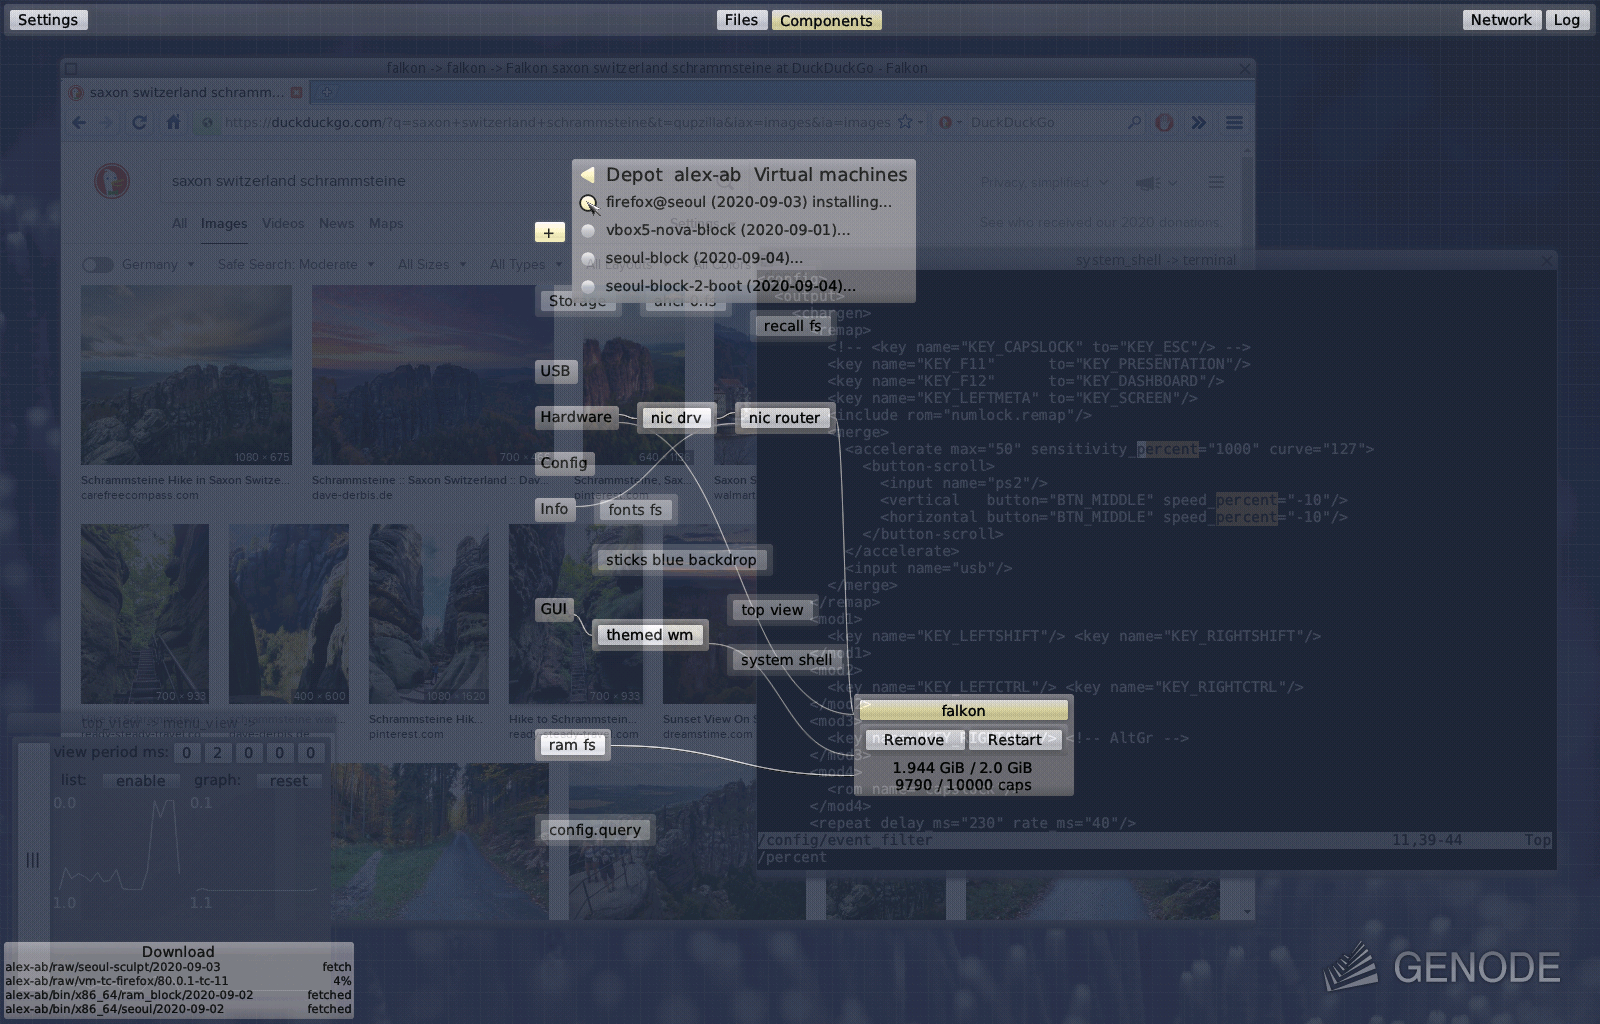
\includegraphics[width=8.0cm]{sculpt_2020-09-16.png}};

	\path (current page.center |- sculptoutline.north)+(4ex,-15ex) node[anchor=north west, screenshot] (phonesection)
		{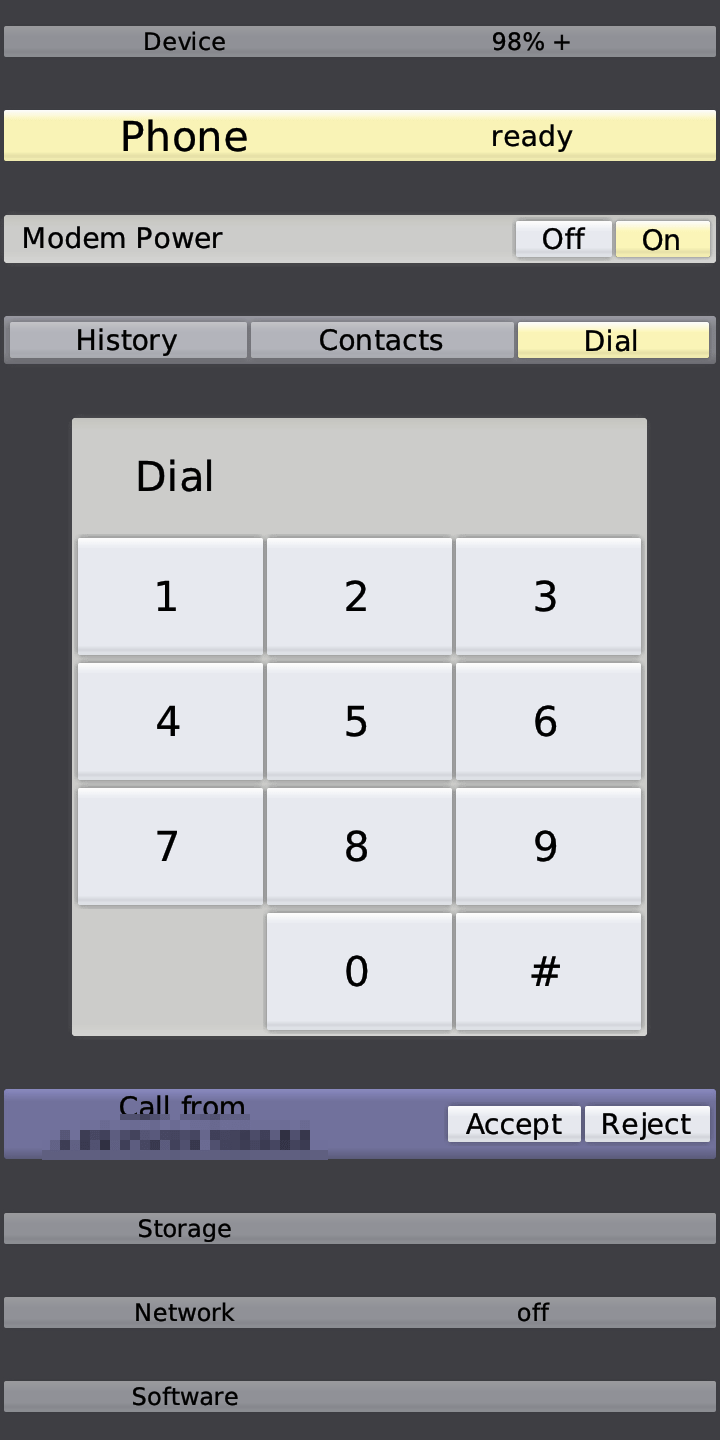
\includegraphics[width=2.5cm]{pinephone_phone_section.png}};

	\path (phonesection.east) node[right=1ex, screenshot] (softwaresection)
		{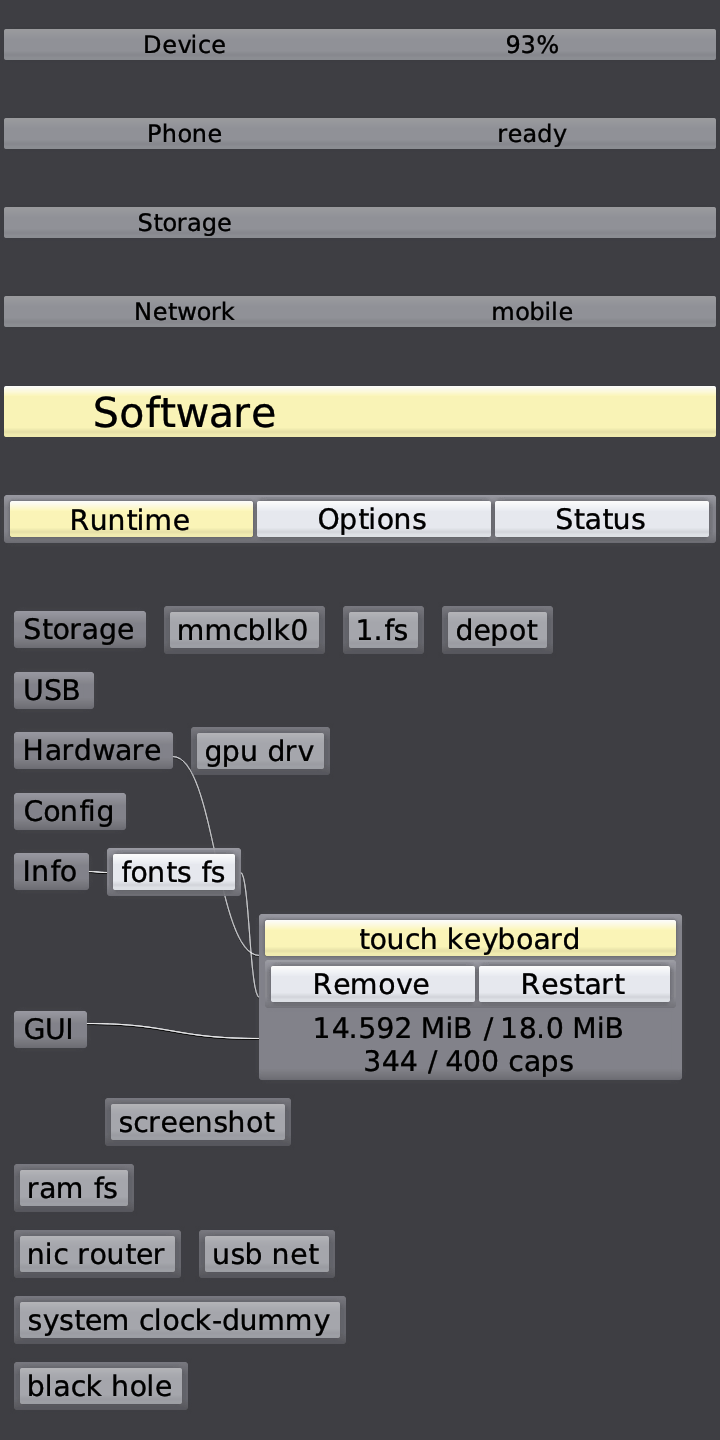
\includegraphics[width=2.5cm]{pinephone_software_section.png}};

	\path (softwaresection.east) node[right=1ex, screenshot] (morph)
		{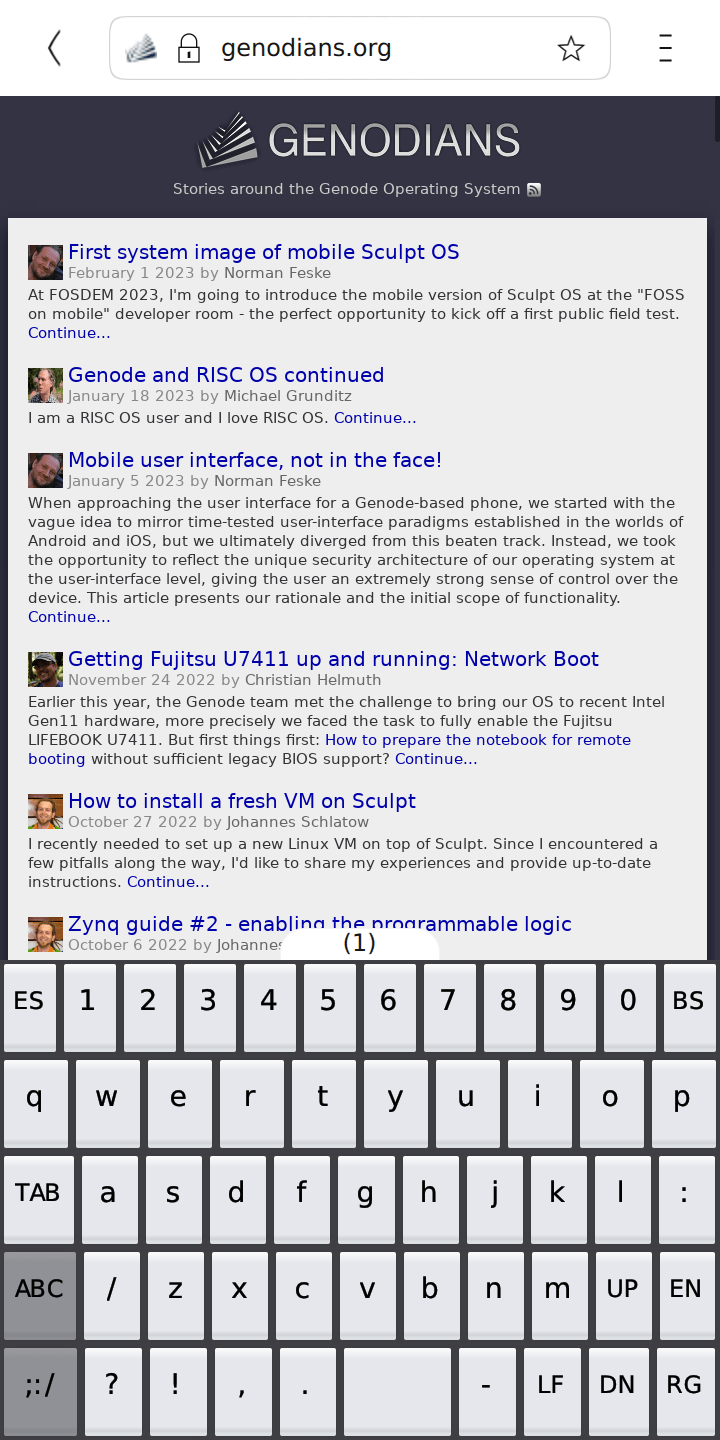
\includegraphics[width=2.5cm]{pinephone_morph.png}};

	\path (sculptpc.north) node[anchor=south, font=\normalsize \sffamily,
	                            color=black, opacity=1, scale=1.2] {Intel PC};

	\path (sculptpc.south) node[inner sep=1ex, anchor=north, font=\normalsize \sffamily,
	                              color=black, opacity=1, scale=1] {VirtualBox available as component};

	\path (softwaresection.south) node[inner sep=1ex, anchor=north, font=\normalsize \sffamily,
	                              color=black, opacity=1, scale=1] {Cold boot takes only 5 seconds};

	\path (softwaresection.north) node[anchor=south, font=\normalsize \sffamily,
	                              color=black, opacity=1, scale=1.2] {PinePhone};

	\path (sculpttitle.south west |- sculptpc.south)+(4ex,-5ex) coordinate (banchor);

	\path (banchor.south west) node[bullet] (banchor) { Attack surface reduced by 99\% };
	\path (banchor.south west) node[bullet] (banchor) {
		Autonomy from dominating software-platform vendors by escaping the security-update treadmill };
	\path (banchor.south west) node[bullet] (banchor) { Integrity-protected on-target package management, system update, and rollback };
	\path (banchor.south west) node[bullet] (banchor) { Security functions: file-encryption vault, WireGuard VPN };
	\path (banchor.south west) node[bullet] (banchor) { Linux drivers as sandboxed components };

	\tikzstyle{wwwlink} = [inner ysep=0.7ex, anchor=east, inner xsep=4ex, font=\normalsize \sffamily,
	                      color=linkcolor, opacity=1, scale=1.2]

	\path (ecooutline.north west)+(4ex,-4ex) coordinate (banchor);
	\path (banchor.south west) node[bullet] (banchor) { Interoperable with POSIX, C++, Qt, GNU, Chromium engine, OpenGL, Java ... };
	\path (banchor.south west) node[bullet] (banchor) { Existing OSes usable as virtual machines };
	\path (banchor.south west) node[bullet] (banchor) { Quarterly releases };
	\path (ecooutline.east |- banchor) node[wwwlink] { https://genode.org };
	\path (banchor.south west) node[bullet] (banchor) { Driven by small team in Germany since 2008 };
	\path (ecooutline.east |- banchor) node[wwwlink] { https://genode-labs.com };
	\path (banchor.south west) node[bullet] (banchor) { Open Source and commercial licensing };
	\path (ecooutline.east |- banchor) node[wwwlink] { https://github.com/genodelabs };
	\path (banchor.south west) node[bullet] (banchor) { International community };
	\path (ecooutline.east |- banchor) node[wwwlink] { https://genodians.org };

	\tikzstyle{userrole} = [inner ysep=3ex, anchor=north, inner xsep=4ex, font=\normalsize \sffamily,
	                      color=white, opacity=1, scale=1.5]

	\path (vendoroutline.north)   node[userrole] (vendor)   {Chip Vendor};
	\path (oemoutline.north)      node[userrole] (oem)      {OEM};
	\path (productoutline.north)  node[userrole] (product)  {Solutions Provider};
	\path (researchoutline.north) node[userrole] (research) {Systems Research};

	\path (vendor.south) node[bullet, anchor=north] { SoC support };
	\path (oem.south) node[bullet, anchor=north] (banchor) { Board support };

	\path (product.south) node[bullet, anchor=north, align=center] { Market-tailored\\ Sculpt OS derivative };


\end{tikzpicture}

\end{titlepage}

\end{document}
